\documentclass[11pt,letterpaper]{article}
\usepackage[utf8]{inputenc}
\usepackage[T1]{fontenc}
\usepackage[margin=2.5cm]{geometry}
\usepackage{amsmath,amssymb,amsthm}
\usepackage{booktabs}
\usepackage{enumitem}
\usepackage{mathptmx}
\usepackage{setspace}
\usepackage{tikz}
\usetikzlibrary{arrows.meta,positioning,calc}
\usepackage{algorithmicx}
\usepackage{algpseudocode}
\usepackage{tcolorbox}
\usepackage[colorlinks=true,linkcolor=blue,citecolor=blue,urlcolor=blue]{hyperref}

\usepackage{xcolor}
\definecolor{azulCambios}{HTML}{289BC3}

% ---------- Portada (estilo minimalista editorial) ----------
\usepackage{graphicx}
\usepackage{tabularx}
\usepackage{colortbl}
% microtype solo se usa para \textls (espaciado entre letras);
% se desactivan protrusion y expansion para no mover el texto
% del resto del reporte.
\usepackage[protrusion=false,expansion=false]{microtype}

\definecolor{ink}{HTML}{2B2B2B}     % texto principal / títulos
\definecolor{muted}{HTML}{7D8A99}   % texto secundario / líneas / labels

% Letra sans de la plantilla original (Latin Modern Sans),
% solo para la portada.
\newcommand{\portadasf}{\fontencoding{T1}\fontfamily{lmss}\selectfont}

% \fieldlabel{TEXTO}: versal pequeña, gris, con tracking.
\newcommand{\fieldlabel}[1]{{\portadasf\small\color{muted}\textls[110]{\MakeUppercase{#1}}}}

\renewcommand{\contentsname}{Índice}
\renewcommand{\abstractname}{Resumen}
\renewcommand{\figurename}{Figura}
\renewcommand{\tablename}{Tabla}
\renewcommand{\appendixname}{Apéndice}
\setstretch{1.08}
\setlength{\parskip}{4pt}
\setlength{\parindent}{0pt}

% ---------- teoremas ----------
\theoremstyle{plain}
\newtheorem{teorema}{Teorema}[section]
\newtheorem{lema}[teorema]{Lema}
\theoremstyle{definition}
\newtheorem{definicion}[teorema]{Definición}
\newtheorem{ejemplo}[teorema]{Ejemplo}
\theoremstyle{remark}
\newtheorem{observacion}[teorema]{Observación}
\renewcommand{\proofname}{Demostración}

% ---------- notación ----------
\newcommand{\C}{\mathcal{C}}
\newcommand{\vacio}{\varnothing}
% Clases y problemas: todos con la misma letra sans de \mathsf
% (Computer Modern Sans), pero como texto, para que en los títulos
% tomen la negrita del título. mathptmx no tiene negritas en
% matemáticas, por eso no se usa \mathsf directamente.
% \upshape evita que salgan en cursiva dentro de los teoremas.
\newcommand{\nombreMat}[1]{\ensuremath{\text{\fontencoding{OT1}\fontfamily{cmss}\upshape\selectfont #1}}}
% Times usa la serie de negritas "b"; Computer Modern Sans solo
% tiene "bx". Se carga la fuente y se declara la equivalencia.
\usefont{OT1}{cmss}{m}{n}
\DeclareFontShape{OT1}{cmss}{b}{n}{<->ssub * cmss/bx/n}{}
\newcommand{\PSPACE}{\nombreMat{PSPACE}}
\newcommand{\NP}{\nombreMat{NP}}
\newcommand{\Pclass}{\nombreMat{P}}
\newcommand{\Pclase}{\nombreMat{P}}
\newcommand{\coNP}{\nombreMat{co-NP}}
\newcommand{\EXPTIME}{\nombreMat{EXPTIME}}
\newcommand{\NPSPACE}{\nombreMat{NPSPACE}}
\newcommand{\QSAT}{\nombreMat{QSAT}}
\newcommand{\PLANNING}{\nombreMat{Planning}}
\newcommand{\Path}{\nombreMat{Path}}

% Versión en texto plano para los marcadores del PDF.
\pdfstringdefDisableCommands{%
  \def\PSPACE{PSPACE}\def\NP{NP}\def\coNP{co-NP}%
  \def\QSAT{QSAT}\def\PLANNING{Planning}\def\Path{Path}%
}
\newcommand{\ptime}{\leq_{\mathrm{P}}}
\newcommand{\cond}[1]{\mathsf{#1}}

% ---------- pseudocódigo en español ----------
\algrenewcommand\algorithmicif{\textbf{si}}
\algrenewcommand\algorithmicthen{\textbf{entonces}}
\algrenewcommand\algorithmicelse{\textbf{si no}}
\algrenewcommand\algorithmicend{\textbf{fin}}
\algrenewcommand\algorithmicfor{\textbf{para}}
\algrenewcommand\algorithmicforall{\textbf{para cada}}
\algrenewcommand\algorithmicdo{\textbf{hacer}}
\algrenewcommand\algorithmicreturn{\textbf{devolver}}
\algrenewtext{EndIf}{\algorithmicend\ \algorithmicif}
\algrenewtext{EndFor}{\algorithmicend\ \algorithmicfor}

% ---------- pasillo del almacén ----------
\newcommand{\pasillo}[4]{%
\begin{tikzpicture}[x=0.9cm,y=0.9cm,baseline=0.2cm]
 \foreach \i/\c in {0/#1,1/#2,2/#3,3/#4}{
  \draw[gray!80] (\i,0) rectangle (\i+1,1);
  \node[font=\scriptsize,gray!70!black] at (\i+0.5,-0.22) {$c_{\number\numexpr\i+1\relax}$};
  \if\c R \node[circle,fill=blue!60!black,text=white,minimum size=5.5mm,inner sep=0pt] at (\i+0.5,0.5) {\small R};\fi
  \if\c B \node[rectangle,fill=green!45!black,text=white,minimum size=5.5mm,inner sep=0pt] at (\i+0.5,0.5) {\small B};\fi
 }
\end{tikzpicture}}

% ---------- Datos editables de la portada ----------
\newcommand{\universidad}{UNAM}
\newcommand{\facultad}{Facultad de Ciencias}
\newcommand{\curso}{Complejidad Computacional}
\newcommand{\tarea}{Reporte \textperiodcentered\ PLANNING}
\newcommand{\profesor}{Carlos Zeron Martinez}
\newcommand{\ayudante}{Malinali Gonzalez Lara}
\newcommand{\fechaentrega}{18 de noviembre de 2026}

% Integrantes del equipo: Nombre & Número de cuenta
\newcommand{\integrantes}{
    Alan Alexzander González Murga & 320079629 \\
    Jesus Antonio Romero Godoy & 321144292 \\
}
% ---------------------------------------------------

\begin{document}

% =====================================================================
% PORTADA
% =====================================================================
\begin{titlepage}
    \color{ink}
    \centering
    \vspace*{1.6cm}

    
\includegraphics[height=2.9cm]{img/escudo-unam.pdf}%
    \hspace{0.8cm}%
    
\includegraphics[height=2.9cm]{img/escudo-facultad.pdf}

    \vspace{1cm}

    \fieldlabel{\universidad\ \textperiodcentered\ \facultad}

    \vspace{\stretch{1}}

    {\color{ink}\rule{0.42\linewidth}{0.6pt}\par}
    \vspace{0.55cm}
    {\portadasf\bfseries\fontsize{30}{34}\selectfont\color{ink}
        \textls[130]{\MakeUppercase{\curso}}\par}
    \vspace{0.35cm}
    {\portadasf\fontsize{14}{16}\selectfont\color{muted}
        \textls[180]{\MakeUppercase{\tarea}}\par}
    \vspace{0.55cm}
    {\color{ink}\rule{0.42\linewidth}{0.6pt}\par}

    \vspace{0.9cm}

    % Título del reporte
    {\Large El problema de planeación (\PLANNING):\\[2pt]
     un problema $\PSPACE$-completo\par}

    \vspace{\stretch{1}}

    \fieldlabel{Integrantes}
    \vspace{0.6cm}

    \renewcommand{\arraystretch}{1.5}
    \begin{tabularx}{0.68\linewidth}{X>{\color{muted}}r}
        \arrayrulecolor{muted}\toprule
        \integrantes
        \arrayrulecolor{muted}\bottomrule
    \end{tabularx}

    \vspace{\stretch{1}}

    \begin{tabular}{r@{\hspace{0.6em}}l}
        \fieldlabel{Profesor:} & \profesor \\[0.35em]
        \fieldlabel{Ayudante:} & \ayudante \\[0.35em]
        \fieldlabel{Fecha de entrega:} & \fechaentrega \\
    \end{tabular}

    \vfill
\end{titlepage}

\tableofcontents
\newpage

% =====================================================================
\section{Introducción}

Gran parte del estudio de la eficiencia algorítmica gira en torno
al tiempo como recurso; así, la distinción entre $\Pclass$ y $\NP$
descansa en esa noción. Sin embargo, la memoria es otro recurso
fundamental, y al tratarla como recurso principal aparece una clase
de problemas que parecen ser incluso más difíciles que $\NP$ y
$\coNP$: la clase $\PSPACE$
(Kleinberg \& Tardos, 2005, p.~531).


\textcolor{azulCambios}{ Uno de los problemas más representativos de PSPACE es el problema de planeación (Planning). De manera general, consiste en determinar si, partiendo de un estado inicial, existe una secuencia de acciones permitidas que permita alcanzar un estado objetivo. }Es el modelo abstracto detrás de la logística de
una operación de socorro, de un robot que acomoda cajas en un
almacén o de los solitarios como el rompecabezas de quince
(Kleinberg \& Tardos, 2005, pp.~533--534). \textcolor{azulCambios}{
Otro ejemplo es la planeación de un viaje con escalas en el que
ciertos vuelos solo pueden tomarse con documentos que se tramitan
en ciertas ciudades, como una visa. Ya no basta con encontrar
conexiones entre ciudades: cada acción cambia las condiciones
del viajero y, con ello, las acciones que tiene disponibles
(véase la sección~\ref{sec:vuelos}).
}

Lo que hace especial a \PLANNING{} es que
\emph{los planes pueden ser exponencialmente largos}, de modo que
ni siquiera es posible escribir una solución completa en espacio
polinomial; aun así, la pregunta de si existe un plan se puede
responder usando solo espacio polinomial.

Nuestro objetivo es presentar \PLANNING{} de forma autocontenida,
por lo que tendremos que definirlo, demostrar que pertenece a
$\PSPACE$ con el algoritmo de Savitch (1970), explicar por qué
es $\PSPACE$-completo, ejecutar el algoritmo en un ejemplo
detallado, y discutir enfoques prácticos, aplicaciones y variantes.

\textbf{Notación.} El libro usa la misma letra $\C$ para el conjunto
de condiciones y para las configuraciones. Aquí escribimos
$c_1,\dots,c_n$ para las condiciones,
$\C=\{c_1,\dots,c_n\}$ para el conjunto de condiciones y
$S, S', S_1, S_2$ para las configuraciones (subconjuntos de $\C$),
con $S_0$ la inicial y $S^{*}$ la meta, para evitar ambigüedades.

% =====================================================================

% =====================================================================
\newpage
\section{Definiciones}

\subsection{La clase $\PSPACE$}

\begin{definicion}[$\PSPACE$]
$\PSPACE$ es el conjunto de problemas que pueden resolverse con
un algoritmo cuyo uso de espacio (memoria) es polinomial en el
tamaño de la entrada
(Kleinberg \& Tardos, 2005, p.~531).
\end{definicion}

En tiempo polinomial un algoritmo solo puede consumir espacio
polinomial, así que

\begin{equation}\label{eq:PsubPSPACE}
\Pclass \subseteq \PSPACE.
\end{equation}

Pero $\PSPACE$ es mucho más amplia. Por ejemplo, un algoritmo
que cuenta de $0$ a $2^{n}-1$ en base $2$ solo necesita un
contador de $n$ bits (como el odómetro de un automóvil);
este se ejecuta en tiempo exponencial pero usa espacio $O(n)$.
La clave de aquí es que \emph{``el espacio se puede reutilizar,
mientras que el tiempo, por definición, no''}
(Kleinberg \& Tardos, 2005, pp.~531--532).

\begin{teorema}[Kleinberg y Tardos, 2005, (9.2)]
\label{teo:3SATpspace}
Existe un algoritmo que resuelve 3-SAT usando solo espacio
polinomial.
\end{teorema}

\begin{proof}
Se recorren todas las asignaciones con un contador de $n$ bits:
cuando el contador vale $q$, la asignación hace $x_i$ igual al
$i$-ésimo bit de $q$. Para cada asignación se evalúa la fórmula
en espacio polinomial; si la satisface, se detiene, y si no,
se borra el trabajo intermedio y se reutiliza ese espacio
para la siguiente asignación.
\end{proof}

\begin{teorema}[Kleinberg y Tardos, 2005, (9.3)]
\label{teo:NPsubPSPACE}
$\NP \subseteq \PSPACE$.
\end{teorema}

\begin{proof}
Si $Y\in\NP$, entonces $Y\ptime$ 3-SAT: hay un algoritmo
para $Y$ que usa un número polinomial de pasos y de llamadas
a una caja negra para 3-SAT. Implementando la caja negra
con el algoritmo del Teorema~\ref{teo:3SATpspace},
se obtiene un algoritmo para $Y$ en espacio polinomial.
\end{proof}

Como $\PSPACE$ es cerrada bajo complemento, también
$\coNP\subseteq\PSPACE$. Además,
$\PSPACE\subseteq\EXPTIME$, porque un algoritmo en espacio
polinomial solo puede visitar un número exponencial de
configuraciones distintas (Sipser, 2013, cap.~8).
La Figura~\ref{fig:jerarquia} resume las contenciones;
no se sabe demostrar que sean estrictas.

% ---------- Figura original: relaciones entre clases ----------
\begin{figure}[ht]
\centering
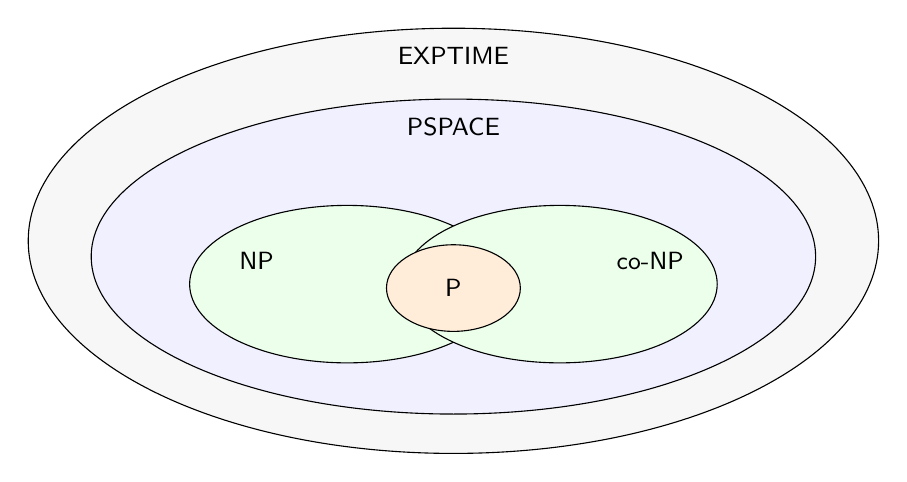
\begin{tikzpicture}[font=\small]
 \draw[fill=gray!6] (0,0) ellipse (5.4 and 2.7);
 \node at (0,2.35) {$\EXPTIME$};

 \draw[fill=blue!6] (0,-0.2) ellipse (4.6 and 2.0);
 \node at (0,1.45) {$\PSPACE$};

 \draw[fill=green!8] (-1.35,-0.55) ellipse (2.0 and 1.0);
 \draw[fill=green!8] (1.35,-0.55) ellipse (2.0 and 1.0);

 \node at (-2.5,-0.25) {$\NP$};
 \node at (2.5,-0.25) {$\coNP$};

 \draw[fill=orange!15] (0,-0.6) ellipse (0.85 and 0.55);
 \node at (0,-0.6) {$\Pclass$};
\end{tikzpicture}
\caption{Relaciones entre clases (basada en
Kleinberg \& Tardos, 2005, Fig.~9.1).}
\label{fig:jerarquia}
\end{figure}

% =====================================================================
\subsection{$\PSPACE$-completitud}

\begin{definicion}[$\PSPACE$-completo]
Un problema $X$ es $\PSPACE$-completo si
(i) $X\in\PSPACE$ y (ii) para todo $Y\in\PSPACE$
se cumple $Y\ptime X$
(Kleinberg \& Tardos, 2005, p.~533).
\end{definicion}

Igual que en $\NP$, si $Y$ es $\PSPACE$-completo
y $X\in\PSPACE$ cumple $Y\ptime X$, entonces $X$
también es $\PSPACE$-completo
(Kleinberg \& Tardos, 2005, p.~544).

El problema ``raíz'' es $\QSAT$ (3-SAT cuantificado),
cuya completitud demostraron Stockmeyer y Meyer (1973).

Por el teorema de Savitch (1970),
$\NPSPACE=\PSPACE$ (Sipser, 2013, teorema~8.5),
lo cual permite trabajar indistintamente con máquinas
deterministas o no deterministas de espacio polinomial.

% =====================================================================
\subsection{Condiciones, operadores y configuraciones}

El modelo de \PLANNING{} es una versión proposicional
del formalismo STRIPS (Fikes \& Nilsson, 1971),
tal como lo presentan Kleinberg y Tardos
(2005, pp.~533--534, 538--539).

\begin{definicion}[Modelo de planeación]\label{def:modelo}
Un modelo de planeación consta de lo siguiente.

\begin{itemize}[leftmargin=1.5em,itemsep=1pt]

\item Un conjunto de \emph{condiciones}
$\C=\{c_1,\dots,c_n\}$.

\item Una \emph{configuración} o \emph{estado}
es un subconjunto $S\subseteq\C$ que representa las
condiciones que se cumplen en un momento dado.

\textcolor{azulCambios}{
Cada condición puede ser verdadera o falsa, por lo que
existen $2^{n}$ configuraciones posibles, correspondientes
a todas las combinaciones de valores verdaderos y falsos
de las $n$ condiciones.
}

\item Un conjunto de \emph{operadores} o \emph{acciones}
$\{O_1,\dots,O_k\}$. Cada $O_i$ tiene una
\emph{lista de prerrequisitos} $P_i\subseteq\C$,
una \emph{lista de adición} $A_i\subseteq\C$
y una \emph{lista de eliminación} $D_i\subseteq\C$.

\item $O_i$ \emph{es aplicable} en $S$ si
$P_i\subseteq S$. Al aplicarlo se obtiene
la configuración

\[
S' \;=\; (S\setminus D_i)\cup A_i .
\]

Se escribe $S\xrightarrow{O_i}S'$.
$O_i$ puede aplicarse aunque haya otras condiciones
además de $P_i$, y no afecta las condiciones que no están
en $A_i$ ni en $D_i$
(Kleinberg \& Tardos, 2005, p.~538).

\end{itemize}
\end{definicion}

\begin{observacion}
El libro no precisa qué ocurre si una condición está a la vez
en $A_i$ y en $D_i$. Aquí se adopta la convención
$S'=(S\setminus D_i)\cup A_i$ (primero se elimina y luego
se agrega); en las construcciones de este reporte las listas
$A_i$ y $D_i$ siempre se toman disjuntas, de modo que
la convención no importa.
\end{observacion}

\begin{ejemplo}[Rompecabezas de quince]
Según el libro, se modela con una condición por cada posible
ubicación de cada ficha y un operador por cada movimiento
de una ficha entre dos ubicaciones adyacentes;
el prerrequisito es que una ubicación contenga a la ficha
y la otra al hueco
(Kleinberg \& Tardos, 2005, p.~534).

Nótese que el modelo no tiene condiciones negativas:
para expresar ``la casilla $c$ está libre'' hace falta
una condición positiva explícita, como
``el hueco está en $c$''.

Se usará el mismo recurso en la aplicación
de la sección~\ref{sec:aplicaciones}.
\end{ejemplo}


% =====================================================================

% =====================================================================
\newpage
\section{Problema de decisión \PLANNING}

\begin{tcolorbox}[
    colback=green!4,
    colframe=green!50!black,
    title=\PLANNING
]
\textbf{Entrada:} un conjunto de condiciones
$\C=\{c_1,\dots,c_n\}$, un conjunto de operadores
o acciones $O_1,\dots,O_k$ con sus respectivas listas
de prerrequisitos, adición y eliminación
$(P_i,A_i,D_i)$, una configuración inicial
$S_0\subseteq\C$ y una configuración meta
$S^{*}\subseteq\C$.\\

\textbf{Pregunta:} ¿existe una secuencia de operadores
$O_{i_1},\dots,O_{i_m}$ tal que, empezando en $S_0$,
cada uno sea aplicable y se llegue exactamente a
$S^{*}$ (es decir, se cumplen precisamente las
condiciones de $S^{*}$ y ninguna otra)?
\end{tcolorbox}


El tamaño de la entrada es polinomial en $n$, $k$
y la longitud de las listas; en particular,
es al menos $n$.

\textcolor{azulCambios}{
Además, como los $k$ operadores se describen explícitamente,
el tamaño de la entrada también es al menos proporcional
a $k$.
}

Un \emph{plan} es una secuencia de operadores que
permite llegar desde la configuración inicial hasta la meta.


\textcolor{azulCambios}{
Sin embargo, \PLANNING{} es un problema de decisión,
por lo que únicamente nos interesa determinar si existe
dicho plan, sin necesidad de construirlo o almacenarlo
completo.
}

\begin{observacion}[Una grafica implícito]

Se puede representar una instancia de \PLANNING{}
mediante una grafica dirigido $\mathcal{G}$, donde cada nodo
representa una de las $2^{n}$ configuraciones posibles
y existe una arista de $S$ a $S'$ si algún operador
permite pasar de una configuración a otra en un solo paso.

De esta manera, \PLANNING{} equivale a preguntar si
\emph{existe un camino en $\mathcal{G}$ desde $S_0$
hasta $S^{*}$}
(Kleinberg \& Tardos, 2005, p.~539).

Aunque $\mathcal{G}$ puede tener un número exponencial
de nodos, está descrito de forma compacta mediante
$n$ condiciones y $k$ operadores.

\textcolor{azulCambios}{
Esto significa que no necesitamos almacenar todas
las configuraciones ni todas las aristas para conocer
las transiciones posibles, ya que podemos calcularlas
a partir de los operadores.
}

\textcolor{azulCambios}{
Por lo tanto, construir explícitamente la grafica completa
puede requerir espacio exponencial, lo que motiva la
búsqueda de un algoritmo capaz de decidir si existe
un camino utilizando únicamente espacio polinomial.
}

\end{observacion}


% =====================================================================

% =====================================================================
\newpage
\section{Planes de longitud exponencial y el procedimiento \Path}

\textcolor{azulCambios}{
Antes de demostrar la complejidad de \PLANNING{}, es necesario
entender por qué los planes pueden ser tan largos y por qué
los algoritmos tradicionales de búsqueda pueden requerir
demasiada memoria. Después presentaremos el procedimiento
\Path, basado en la técnica de Savitch, que permite decidir
si existe un plan sin almacenarlo completo.
}

\subsection{Planes de longitud exponencial}

En algunas instancias hay planes cortos (como en el
rompecabezas de quince), pero esto no ocurre en general.

\begin{teorema}[Kleinberg y Tardos, 2005, (9.6)]
\label{teo:96}
Existen instancias de \PLANNING{} con $n$ condiciones
y $n$ operadores que tienen solución, pero cuyo plan
más corto tiene longitud $2^{n}-1$.
\end{teorema}

\begin{proof}
La instancia codifica el incremento de un contador
de $n$ bits desde todos ceros hasta todos unos.

\begin{itemize}[leftmargin=1.5em,itemsep=1pt]
\item Condiciones $c_1,\dots,c_n$ y operadores
$O_1,\dots,O_n$.

\item $O_1$ no tiene prerrequisitos ni lista de
eliminación; solo agrega $c_1$.

\item Para $i>1$, $O_i$ requiere $c_j$ para todo
$j<i$; al invocarse agrega $c_i$ y elimina
$c_j$ para todo $j<i$.

\item $S_0=\vacio$ y $S^{*}=\{c_1,\dots,c_n\}$.
\end{itemize}

Se afirma, por inducción sobre $i$, lo siguiente:
\emph{desde cualquier configuración que no contenga
ningún $c_j$ con $j\le i$, existe una secuencia
de operadores que llega a una configuración que
contiene a todos los $c_j$ con $j\le i$, y toda
secuencia así tiene al menos $2^{i}-1$ pasos.}

Para $i=1$ es claro. Para $i>1$ hay una solución:
(1) por inducción se logran
$\{c_{i-1},\dots,c_1\}$ con
$O_1,\dots,O_{i-1}$;
(2) se invoca $O_i$, que agrega $c_i$ y elimina
todos los demás;
(3) por inducción se logran de nuevo
$\{c_{i-1},\dots,c_1\}$, y $c_i$ se conserva.

Para la cota inferior, considérese el primer momento
en que se agrega $c_i$. Solo $O_i$ puede agregarla,
y para invocarlo deben estar presentes
$c_{i-1},\dots,c_1$, lo que por inducción requirió
al menos $2^{i-1}-1$ pasos. Pero $O_i$ elimina todos
los $c_j$ con $j<i$, así que hay que lograrlos otra vez,
lo que requiere otros $2^{i-1}-1$ pasos.

En total, al menos
$2(2^{i-1}-1)+1=2^{i}-1$ pasos.
Aplicando la afirmación con $i=n$ se obtiene
el resultado.
\end{proof}

\begin{ejemplo}[$n=3$]
El plan más corto tiene $7$ pasos:
$O_1,O_2,O_1,O_3,O_1,O_2,O_1$,
que recorre las configuraciones

\[
\vacio\to\{c_1\}\to\{c_2\}
\to\{c_1,c_2\}\to\{c_3\}
\to\{c_1,c_3\}\to\{c_2,c_3\}
\to\{c_1,c_2,c_3\}.
\]

(Es exactamente la cuenta en binario con el bit
menos significativo a la izquierda.)
Este plan fue verificado con el programa del
apéndice~A.
\end{ejemplo}

\subsection{Cota superior sobre la longitud}

\begin{teorema}[Kleinberg y Tardos, 2005, (9.7)]
\label{teo:97}
Si una instancia de \PLANNING{} con $n$ condiciones
tiene solución, entonces tiene una con a lo más
$2^{n}-1$ pasos.
\end{teorema}

\begin{proof}
La grafica $\mathcal{G}$ tiene $2^{n}$ nodos.
Si hay un camino de $S_0$ a $S^{*}$, el más corto
no visita ningún nodo más de una vez; por tanto,
tiene a lo más $2^{n}-1$ aristas.
\end{proof}

\begin{observacion}[Consecuencia: el plan no sirve como certificado]
Si todo plan tuviera longitud polinomial,
bastaría exhibirlo y \PLANNING{} estaría en $\NP$.
Pero el Teorema~\ref{teo:96} muestra que el plan
más corto puede ser exponencial, así que no es
un buen certificado.

Además, en espacio polinomial ni siquiera se puede
almacenar una representación explícita de la solución
(Kleinberg \& Tardos, 2005, p.~540).
La pregunta es entonces si se puede \emph{decidir}
la existencia de un plan sin tener nunca la
solución completa a la vista.

\textcolor{azulCambios}{
Esto no demuestra que \PLANNING{} esté fuera de
$\NP$, sino que una secuencia explícita de acciones
no siempre constituye un certificado de tamaño
polinomial.
}
\end{observacion}

\subsection{Enfoques exponenciales}\label{sec:enfoquesexp}

Un primer algoritmo construye $\mathcal{G}$ y aplica
búsqueda en profundidad (DFS) o en amplitud (BFS)
desde $S_0$. Esto toma espacio exponencial solo
para construir la grafica.

Se podría simular DFS o BFS sin construir
$\mathcal{G}$, pero tampoco es viable: DFS debe
mantener la lista de nodos del camino actual y
BFS la de la frontera, y ambas pueden crecer de
forma exponencial
(Kleinberg \& Tardos, 2005, p.~541).

Hace falta un algoritmo de búsqueda de caminos
fundamentalmente distinto.

\subsection{El procedimiento \Path}\label{sec:path}

La idea, propuesta por Savitch (1970), es aplicar
divide y vencerás sobre la \emph{longitud} del camino.

Se define $\Path(S_1,S_2,L)$ como el procedimiento
que decide si existe una secuencia de \emph{a lo más}
$L$ operadores que lleve de la configuración $S_1$
a la configuración $S_2$.

El problema original es
$\Path(S_0,S^{*},2^{n})$, lo cual es suficiente
por el Teorema~\ref{teo:97}.

En lugar de hacer crecer el camino de uno en uno
(como BFS), se parte en dos mitades de a lo más
$\lceil L/2\rceil$ pasos cada una, unidas por un
\emph{punto medio} $S'$
(Kleinberg \& Tardos, 2005, p.~541).

\textcolor{azulCambios}{
El procedimiento prueba las configuraciones posibles
como puntos medios, una por una. Para cada candidata,
primero comprueba si existe un camino desde $S_1$
hasta ella y después si existe uno desde ella hasta
$S_2$. Si ambas respuestas son afirmativas, existe
un camino entre las configuraciones originales.
Al terminar cada llamada recursiva se reutiliza su
memoria, conservando únicamente el resultado necesario.
}

\begin{tcolorbox}[
colback=gray!5,
colframe=gray!60,
title={Procedimiento $\Path(S_1,S_2,L)$
(Kleinberg \& Tardos, 2005, p.~542)}
]
\begin{algorithmic}[1]
\Statex \textbf{Entrada:} configuraciones $S_1,S_2$
y un entero $L$ (potencia de $2$).

\If{$L=1$}
    \If{$S_1=S_2$ o hay un operador $O$
    que convierte $S_1$ en $S_2$}
        \State \Return ``sí''
    \Else
        \State \Return ``no''
    \EndIf
\Else
    \State Enumerar todas las configuraciones
    $S'$ con un contador de $n$ bits.
    \ForAll{$S'$}
        \State $x \gets
        \Path(S_1,S',\lceil L/2\rceil)$;
        borrar todo el trabajo intermedio salvo $x$.

        \State $y \gets
        \Path(S',S_2,\lceil L/2\rceil)$;
        borrar todo el trabajo intermedio salvo $y$.

        \If{$x=$ ``sí'' y $y=$ ``sí''}
            \State \Return ``sí''
        \EndIf
    \EndFor
    \State \Return ``no''
\EndIf
\end{algorithmic}
\end{tcolorbox}

\begin{observacion}[Adaptaciones menores]
(1) El libro escribe el caso base solo con la condición
``hay un operador que convierte $S_1$ en $S_2$'';
aquí se agrega ``$S_1=S_2$'' para que $\Path$
signifique literalmente ``a lo más $L$ pasos''
(permite la secuencia vacía).

(2) El pseudocódigo calcula siempre $x$ y $y$;
si $x=$ ``no'' se puede omitir el cálculo de $y$
sin afectar la correctitud ni el espacio.
El ejemplo de la sección~\ref{sec:ejemplo}
usa esta optimización.

(3) Hay que recordar que $L$ es un parámetro
exponencialmente grande: $\log L=n$.
\end{observacion}


% =====================================================================

\newpage
% =====================================================================
\section{Demostración de que \PLANNING{} pertenece a $\PSPACE$}

\textcolor{azulCambios}{
Para demostrar que \PLANNING{} pertenece a $\PSPACE$,
necesitamos justificar dos propiedades del procedimiento
\Path: primero, que responde correctamente si existe
un plan y, segundo, que utiliza una cantidad de
memoria polinomial respecto al tamaño de la entrada.
}

\subsection{Correctitud}

\begin{teorema}[Kleinberg y Tardos, 2005, (9.8), correctitud]
\label{teo:98c}
$\Path(S_1,S_2,L)$ devuelve ``sí'' si y solo si
existe una secuencia de a lo más $L$ operadores
que lleva de $S_1$ a $S_2$.
\end{teorema}

\begin{proof}
Por inducción sobre $L$ (potencia de $2$).
Si $L=1$, el algoritmo revisa explícitamente
todos los operadores (y el caso $S_1=S_2$),
así que es correcto.

Sea $L>1$.

($\Leftarrow$)
Si existe una secuencia de longitud $L'\le L$
de $S_1$ a $S_2$, sea $S'$ la configuración que
ocurre en la posición $\lceil L'/2\rceil$
de la secuencia.

El tramo de $S_1$ a $S'$ tiene longitud
$\lceil L'/2\rceil\le\lceil L/2\rceil$
y el tramo de $S'$ a $S_2$ tiene longitud
$L'-\lceil L'/2\rceil\le\lceil L/2\rceil$.

Por hipótesis de inducción,
$\Path(S_1,S',\lceil L/2\rceil)$ y
$\Path(S',S_2,\lceil L/2\rceil)$ devuelven
``sí''; como el ciclo prueba todas las
configuraciones, en algún momento llega a
este $S'$ y el procedimiento devuelve ``sí''.

($\Rightarrow$)
Si devuelve ``sí'', existe $S'$ con ambas
llamadas en ``sí''. Por hipótesis de inducción
hay una secuencia de a lo más $\lceil L/2\rceil$
operadores de $S_1$ a $S'$ y otra de a lo más
$\lceil L/2\rceil$ de $S'$ a $S_2$.

Al concatenarlas se obtiene una secuencia
de a lo más $L$ operadores de $S_1$ a $S_2$.
\end{proof}

\subsection{Espacio polinomial}

\begin{teorema}[Kleinberg y Tardos, 2005, (9.8), espacio]
\label{teo:98e}
El espacio que usa $\Path(S_1,S_2,L)$ es polinomial
en $n$, $k$ y $\log L$. En particular,
$\Path(S_0,S^{*},2^{n})$ usa espacio polinomial
en $n$ y $k$.
\end{teorema}

\begin{proof}
Sin contar el espacio de las llamadas recursivas,
cada invocación usa una cantidad de espacio
polinomial en $n$, $k$ y $\log L$.

En cada momento hay una única llamada recursiva
activa: el trabajo intermedio de las demás ya se
borró, y de ellas solo se conserva un bit.

Por tanto, para un polinomio $p$, el espacio
$S(n,k,L)$ satisface

\[
S(n,k,L)\le
p(n,k,\log L)+S(n,k,\lceil L/2\rceil),
\qquad
S(n,k,1)\le p(n,k,1).
\]

Al desenrollar la recurrencia durante
$O(\log L)$ niveles se obtiene

\[
S(n,k,L)=O(\log L\cdot p(n,k,\log L)),
\]

que es polinomial en $n$, $k$ y $\log L$.
\end{proof}

\paragraph{Cuenta explícita de la pila.}
Un marco de $\Path$ guarda:
$S_1$, $S_2$ y $S'$ ($n$ bits cada uno),
el contador que enumera las configuraciones
($n$ bits), el exponente $j$ con $L=2^{j}$
($O(\log n)$ bits) y los bits $x,y$.

Para decidir si un operador convierte
$S_1$ en $S_2$ se recorren las listas de
la entrada, con $O(n+\log k)$ bits adicionales.

Cada marco usa entonces $O(n+\log k)$ bits.
Como $L$ se divide entre $2$ en cada nivel,
desde $2^{n}$ hasta $1$, la profundidad
de la recursión es $n+1$.

El espacio total es
$O\bigl(n(n+\log k)\bigr)$ bits,
más la entrada (que se lee pero no se copia).
\textcolor{azulCambios}{Como el tamaño de la entrada
es al menos $n$ y al menos proporcional a $k$,
esta cota es polinomial en el tamaño de la entrada.}

\subsection{Tiempo de ejecución}

El espacio se ahorra a costa de tiempo.
Sea $N(L)$ el número de llamadas a $\Path$
que genera una llamada con parámetro $L$.

El ciclo recorre $2^{n}$ configuraciones
y hace a lo más dos llamadas por cada una, así que

\[
N(1)=1,\qquad
N(L)\le 1+2^{n+1}N(L/2).
\]

Con $a=2^{n+1}$ y $L=2^{j}$ resulta

\[
N(2^{j})\le\sum_{i=0}^{j}a^{i}\le 2a^{j},
\]

y por tanto

\[
N(2^{n})\;\le\;2\cdot 2^{n(n+1)}
\;=\;2^{O(n^{2})}.
\]

Cada llamada cuesta tiempo polinomial, de modo
que el tiempo total es $2^{O(n^{2})}$:
exponencial, pero con espacio polinomial.

Esto es lo opuesto a la programación dinámica,
cuyo principio es guardar todo el trabajo
intermedio para no recalcularlo; aquí se tira
todo y se recalcula
(Kleinberg \& Tardos, 2005, p.~543).

\subsection{Conclusión: pertenencia a $\PSPACE$}

\begin{teorema}\label{teo:planningPSPACE}
$\PLANNING\in\PSPACE$.
\end{teorema}

\begin{proof}
Por los Teoremas~\ref{teo:97},
\ref{teo:98c} y~\ref{teo:98e}:
$\Path(S_0,S^{*},2^{n})$ decide la
instancia y usa espacio polinomial.
\end{proof}


% =====================================================================


% =====================================================================
\newpage
\section{Demostración de la $\PSPACE$-completitud de
\PLANNING{}}\label{sec:completitud}

{\color{azulCambios}
En la sección anterior demostramos que
$\PLANNING\in\PSPACE$. Sin embargo, para concluir
que es $\PSPACE$-completo también debemos
demostrar que es $\PSPACE$-difícil.

Esto requiere mostrar que cualquier problema
de $\PSPACE$ puede reducirse en tiempo polinomial
a una instancia de \PLANNING{}.
}

\subsection{$\PSPACE$-dificultad y relación con $\QSAT$}

El libro observa que la $\PSPACE$-dificultad
se puede probar mediante
una reducción desde $\QSAT$, pero no desarrolla
la prueba (Kleinberg \& Tardos, 2005, p.~544).

$\QSAT$ pregunta si
$\exists x_1\,\forall x_2\cdots\exists x_n\;
\Phi(x_1,\dots,x_n)$ es verdadera, con $\Phi$
una conjunción de cláusulas de tres términos;
su $\PSPACE$-completitud se debe a Stockmeyer
y Meyer (1973)
(Kleinberg \& Tardos, 2005, p.~543).

Que la planeación sea difícil se entiende bien
por esta conexión: $\QSAT$ modela la planeación
de contingencias, en la que se pregunta si hay
una decisión tal que \emph{para toda} respuesta
hay otra decisión, y así sucesivamente
(Kleinberg \& Tardos, 2005, p.~535).

La completitud de \PLANNING{} fue establecida por
Bylander (1994), quien muestra que decidir la
existencia de un plan en STRIPS proposicional es
$\PSPACE$-completo en general; su demostración
de dureza codifica una máquina de Turing mediante
operadores STRIPS
(véase la descripción en Edelkamp et~al., 2026).

\textcolor{azulCambios}{
La dureza se demuestra con la reducción de la
siguiente sección.
}

\subsection{Reducción desde máquinas de Turing de espacio polinomial}
\label{sec:reduccion}

Esta sección es un esbozo propio, que sigue la técnica
estándar de simular un cómputo con condiciones
y operadores; la prueba original y sus variantes
están en Bylander (1994).

\subsubsection{Idea}

Sea $A\in\PSPACE$ decidido por una máquina
de Turing determinista
$M=(Q,\Sigma,\Gamma,\delta,q_0,q_{\mathrm{acc}})$
que usa a lo más $p(|w|)$ celdas con $p$ un polinomio.

Dada una entrada $w$ con $|w|=m$ y $s=p(m)$,
se construye una instancia de \PLANNING{}
cuyas configuraciones representan las
configuraciones instantáneas de $M$.

Cada transición de $M$ se convierte en un
operador. Entonces $M$ acepta $w$ si y
solo si existe un plan.

Sin pérdida de generalidad se supone que,
antes de aceptar, $M$ borra la cinta
(la llena de blancos $\sqcup$) y regresa
la cabeza a la celda~$1$; esto no aumenta
el espacio.

\textcolor{azulCambios}{
También sin pérdida de generalidad, $M$ nunca intenta
moverse a la izquierda desde la celda~$1$ ni a la derecha
desde la celda~$s$. Por eso basta definir operadores
para las posiciones $i$ con $1\le i+D\le s$.
}

Así, la configuración aceptora es única,
lo que permite expresarla como la meta
\emph{exacta} que exige el problema.

\subsubsection{Construcción}

\begin{itemize}[leftmargin=1.5em,itemsep=2pt]

\item \textbf{Condiciones.}
$\cond{Q}_q$ para cada estado $q\in Q$
(``la máquina está en el estado $q$'');
$\cond{H}_i$ para $1\le i\le s$
(``la cabeza está en la celda $i$'');
y $\cond{S}_{i,a}$ para $1\le i\le s$
y $a\in\Gamma$
(``la celda $i$ contiene a $a$'').

En total,
$n=|Q|+s+s|\Gamma|$ condiciones.

\item \textbf{Operadores.}
Por cada transición
$\delta(q,a)=(q',b,D)$
con $D\in\{-1,+1\}$ y cada posición
$i$ tal que $1\le i+D\le s$,
un operador $O_{q,a,i}$ con

\[
P=\{\cond{Q}_q,\cond{H}_i,\cond{S}_{i,a}\},
\]

\[
A=\{\cond{Q}_{q'},\cond{H}_{i+D},\cond{S}_{i,b}\},
\]

\[
D_{\mathrm{el}}=
\{\cond{Q}_q,\cond{H}_i,\cond{S}_{i,a}\}.
\]

Si alguna condición aparece a la vez en $A$
y en la lista de eliminación
(por ejemplo, si $q'=q$ o $b=a$),
se quita de ambas listas; así quedan
disjuntas y la condición sigue cumpliéndose
porque estaba en $P$.

\item \textbf{Configuración inicial.}

\[
S_0=
\{\cond{Q}_{q_0},\cond{H}_1\}
\cup
\{\cond{S}_{i,w_i}:1\le i\le m\}
\cup
\{\cond{S}_{i,\sqcup}:m<i\le s\}.
\]

\item \textbf{Meta.}

\[
S^{*}=
\{\cond{Q}_{q_{\mathrm{acc}}},\cond{H}_1\}
\cup
\{\cond{S}_{i,\sqcup}:1\le i\le s\}.
\]

\end{itemize}

\begin{ejemplo}
La transición
$\delta(q_1,0)=(q_2,1,+1)$
en la posición $i$ da el operador con

\[
P=\{\cond{Q}_{q_1},\cond{H}_i,\cond{S}_{i,0}\},
\]

adiciones

\[
\{\cond{Q}_{q_2},\cond{H}_{i+1},\cond{S}_{i,1}\}
\]

y eliminaciones

\[
\{\cond{Q}_{q_1},\cond{H}_i,\cond{S}_{i,0}\}.
\]

Cambia de estado, escribe un $1$ y mueve
la cabeza una celda a la derecha.
\end{ejemplo}

\subsubsection{Tiempo de construcción}

Hay $n=|Q|+s(1+|\Gamma|)$ condiciones
y a lo más $|\delta|\cdot s$ operadores,
cada uno con a lo más tres elementos en
cada lista.

Como $M$ es fija y $s=p(m)$ es un polinomio,
la instancia tiene tamaño polinomial en $m$
y se construye en tiempo polinomial.

\subsubsection{Correctitud}

\textbf{Invariante.}
En toda configuración alcanzable desde $S_0$
hay exactamente una condición $\cond{Q}_q$,
exactamente una $\cond{H}_i$ y,
para cada celda $i$, exactamente una
$\cond{S}_{i,a}$.

Es cierto en $S_0$ y cada operador lo preserva
(elimina una de cada tipo y agrega una de cada tipo).

Por el invariante, cada configuración alcanzable
codifica una configuración instantánea de $M$.

\begin{itemize}[leftmargin=1.5em,itemsep=2pt]

\item[($\Rightarrow$)]
Si $M$ acepta $w$, su cómputo es una sucesión
de configuraciones instantáneas que no sale
de las celdas $1..s$ y termina en la
configuración aceptora.

Aplicando en orden los operadores $O_{q,a,i}$
de las transiciones usadas, se obtiene un plan
de $S_0$ a $S^{*}$.

\item[($\Leftarrow$)]
Si hay un plan, por el invariante en cada paso
el único operador aplicable es el que corresponde
a $(q,a,i)$ de la configuración actual
(la máquina es determinista), así que el plan
reproduce el cómputo de $M$ sobre $w$ y alcanza
$S^{*}$, es decir, la configuración aceptora.

Luego $M$ acepta $w$.

\end{itemize}

Como $M$ siempre se detiene, el plan existe
si y solo si $w\in A$.

Se concluye que $A\ptime\PLANNING$ para
todo $A\in\PSPACE$.

\subsection{Conclusión: $\PSPACE$-completitud}

{\color{azulCambios}
La reducción anterior demuestra que
\PLANNING{} es $\PSPACE$-difícil, pues permite
transformar cualquier problema de $\PSPACE$
en una instancia equivalente de planeación
en tiempo polinomial.

Como también demostramos que
$\PLANNING\in\PSPACE$, se cumplen las dos
condiciones necesarias para establecer
su $\PSPACE$-completitud.
}

\begin{teorema}[Bylander, 1994]
$\PLANNING{}$ es $\PSPACE$-completo.
\end{teorema}

% =====================================================================
\newpage
\section{Ejemplo de la ejecución del algoritmo}\label{sec:ejemplo}

Se usa la instancia del contador de $n=2$ bits del Teorema~\ref{teo:96}. Todos los resultados de esta sección fueron verificados con el programa del apéndice~A.

\subsection{La instancia}

\begin{itemize}[leftmargin=1.5em,itemsep=1pt]
\item Condiciones $c_1,c_2$ ($n=2$, así que $L=2^{2}=4$) y $2^{2}=4$ configuraciones.
\item $O_1$: $P_1=\vacio$, $A_1=\{c_1\}$, $D_1=\vacio$.
\item $O_2$: $P_2=\{c_1\}$, $A_2=\{c_2\}$, $D_2=\{c_1\}$.
\item $S_0=\vacio$ y $S^{*}=\{c_1,c_2\}$; se escribe $M=\{c_1,c_2\}$ para la meta.
\end{itemize}
Se espera un plan de $2^{2}-1=3$ pasos. La pregunta es si $\Path(\vacio,M,4)$ devuelve ``sí''.

\subsection{La grafica implícita $\mathcal{G}$}

El algoritmo \emph{nunca construye} esta grafica; se muestra solo para seguir su razonamiento.

\begin{figure}[ht]
\centering
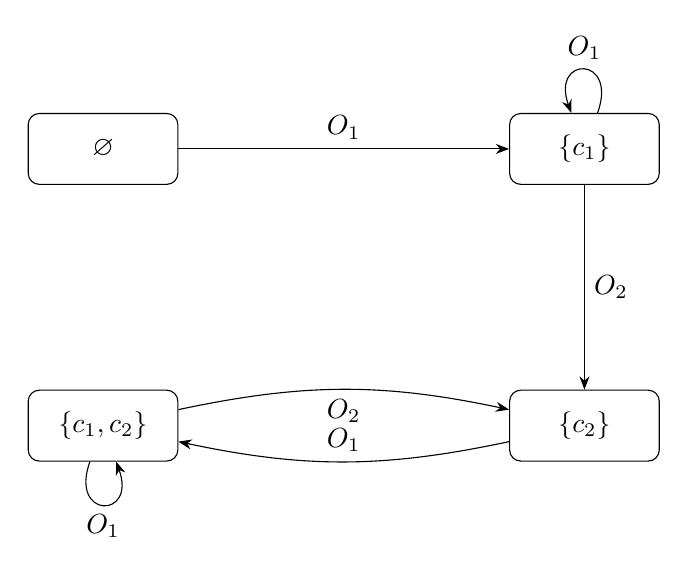
\begin{tikzpicture}[>=Stealth,node distance=4.2cm,auto,
  est/.style={draw,rounded corners,minimum width=1.9cm,minimum height=0.9cm}]
 \node[est] (e)  {$\vacio$};
 \node[est,right=of e]  (c1) {$\{c_1\}$};
 \node[est,below=2.6cm of c1] (c2) {$\{c_2\}$};
 \node[est,below=2.6cm of e] (c12) {$\{c_1,c_2\}$};
 \draw[->] (e) -- node {$O_1$} (c1);
 \draw[->] (c1) -- node {$O_2$} (c2);
 \draw[->,bend left=12] (c2) to node[swap] {$O_1$} (c12);
 \draw[->,bend left=12] (c12) to node[swap] {$O_2$} (c2);
 \draw[->] (c1) to[out=70,in=110,looseness=6] node[above] {$O_1$} (c1);
 \draw[->] (c12) to[out=250,in=290,looseness=6] node[below] {$O_1$} (c12);
\end{tikzpicture}
\caption{Grafica de configuraciones del contador de $2$ bits. El plan de $3$ pasos es $\vacio\xrightarrow{O_1}\{c_1\}\xrightarrow{O_2}\{c_2\}\xrightarrow{O_1}\{c_1,c_2\}$.}
\end{figure}

El operador $O_2$ no es aplicable en $\vacio$ ni en $\{c_2\}$ (falta $c_1$). El contador de $n=2$ bits enumera las configuraciones en este orden: $\vacio,\{c_1\},\{c_2\},\{c_1,c_2\}$ (el bit $i$ del contador indica si $c_i$ pertenece).

\subsection{Ejecución de $\Path(\vacio,M,4)$}

Como $L=4>1$, se prueban los puntos medios $S'$ en orden, con $\lceil L/2\rceil=2$:

\begin{center}
\begin{tabular}{@{}lllc@{}}
\toprule
$S'$ & $x=\Path(\vacio,S',2)$ & $y=\Path(S',M,2)$ & Resultado\\
\midrule
$\vacio$ & sí & no & se descarta\\
$\{c_1\}$ & sí & sí & \textbf{sí}\\
\bottomrule
\end{tabular}
\end{center}
Como ya se encontró un $S'$ con ambas respuestas en ``sí'', el ciclo se detiene y no se prueban $\{c_2\}$ ni $M$. A continuación se detalla cada fila (en cada subllamada, $\lceil 2/2\rceil=1$).

\paragraph{Fila $S'=\vacio$.} $x=\Path(\vacio,\vacio,2)$ es ``sí'': con $S''=\vacio$, ambas llamadas $\Path(\vacio,\vacio,1)$ son ``sí'' porque $S_1=S_2$.
Para $y=\Path(\vacio,M,2)$ se prueban los puntos medios $S''$:

\begin{center}
\begin{tabular}{@{}lll@{}}
\toprule
$S''$ & $\Path(\vacio,S'',1)$ & $\Path(S'',M,1)$\\
\midrule
$\vacio$ & sí ($S_1=S_2$) & no ($O_1$ lleva $\vacio$ a $\{c_1\}$, no a $M$)\\
$\{c_1\}$ & sí ($O_1$) & no ($O_1\to\{c_1\}$, $O_2\to\{c_2\}$)\\
$\{c_2\}$ & no & no se evalúa\\
$M$ & no & no se evalúa\\
\bottomrule
\end{tabular}
\end{center}
Ningún $S''$ sirve, así que $y=$ ``no''. Es coherente: el camino más corto de $\vacio$ a $M$ mide $3$ pasos, no $2$.

\paragraph{Fila $S'=\{c_1\}$.} $x=\Path(\vacio,\{c_1\},2)$ es ``sí'': con $S''=\vacio$, $\Path(\vacio,\vacio,1)=$ ``sí'' y $\Path(\vacio,\{c_1\},1)=$ ``sí'' por $O_1$.
Para $y=\Path(\{c_1\},M,2)$:

\begin{center}
\begin{tabular}{@{}lll@{}}
\toprule
$S''$ & $\Path(\{c_1\},S'',1)$ & $\Path(S'',M,1)$\\
\midrule
$\vacio$ & no & no se evalúa\\
$\{c_1\}$ & sí ($S_1=S_2$) & no\\
$\{c_2\}$ & sí ($O_2$) & sí ($O_1$: $\{c_2\}\to\{c_1,c_2\}$)\\
\bottomrule
\end{tabular}
\end{center}
Con $S''=\{c_2\}$ ambas llamadas dan ``sí'', así que $y=$ ``sí''.

\paragraph{Resultado.} $\Path(\vacio,M,4)=$ ``sí''. De la ejecución se puede leer el plan $\vacio\xrightarrow{O_1}\{c_1\}\xrightarrow{O_2}\{c_2\}\xrightarrow{O_1}\{c_1,c_2\}$, aunque el algoritmo solo devuelve el bit de respuesta.
En total hubo $20$ llamadas a $\Path$ con la optimización de omitir $y$ cuando $x=$ ``no'' ($23$ sin ella).

\subsection{Estado de la memoria}

En el punto más profundo de la ejecución, la pila contiene tres marcos, no más:
\begin{enumerate}[leftmargin=2em,itemsep=1pt]
\item $\Path(\vacio,M,4)$, con $S'=\{c_1\}$;
\item $\Path(\{c_1\},M,2)$, con $S''=\{c_2\}$;
\item $\Path(\{c_2\},M,1)$.
\end{enumerate}
Cuando termina una llamada se libera su marco y solo sobrevive un bit. En ningún momento se guardó el plan completo, que sería lo que exige tanto espacio en un enfoque con DFS o BFS.

\subsection{¿Qué pasa cuando $n$ crece?}

La Tabla~\ref{tab:escala} muestra el costo para el contador de $n$ bits. La pila crece linealmente, mientras que el número de llamadas crece muy rápido (cota teórica $2^{O(n^{2})}$).

\begin{table}[ht]
\centering
\begin{tabular}{@{}rrrrr@{}}
\toprule
$n$ & Nodos de $\mathcal{G}$ ($2^{n}$) & Pasos del plan mínimo ($2^{n}-1$) & Marcos de pila ($n+1$) & Llamadas a $\Path$\\
\midrule
2 & 4 & 3 & 3 & 20\\
3 & 8 & 7 & 4 & 454\\
4 & 16 & 15 & 5 & 48\,795\\
5 & 32 & 31 & 6 & 23\,167\,425\\
\bottomrule
\end{tabular}
\caption{Resultados medidos con el programa del apéndice~A (con la optimización de omitir $y$). Para cada $n$, $\Path(\vacio,\{c_1,\dots,c_n\},2^{n})$ devolvió ``sí'' y la longitud mínima, calculada con BFS, coincidió con $2^{n}-1$.}
\label{tab:escala}
\end{table}

Para $n=60$ el plan mínimo tendría $2^{60}-1\approx1.15\times10^{18}$ pasos, pero la pila tendría solo $61$ marcos de $O(n)$ bits: del orden de unos cuantos miles de bits. Ese es el intercambio entre tiempo y espacio.

% =====================================================================
\section{Enfoques para resolver el problema}

\begin{table}[ht]
\centering
\small
\begin{tabular}{@{}p{3.3cm}p{3.2cm}p{3.5cm}p{4.4cm}@{}}
\toprule
Enfoque & Espacio & Tiempo & Comentario\\
\midrule
BFS/DFS sobre $\mathcal{G}$ & $2^{O(n)}$ & $2^{O(n)}$ (poly en $|\mathcal{G}|$) & Es el más rápido, pero inviable en memoria para $n$ grande.\\
$\Path$ (Savitch) & polinomial, $O(n(n+\log k))$ bits & $2^{O(n^{2})}$ & Prueba que \PLANNING{} $\in\PSPACE$; no se usa en la práctica.\\
Planificadores prácticos & depende del dominio & sin garantía en el peor caso & Heurísticas y codificaciones; resuelven muchas instancias grandes.\\
\bottomrule
\end{tabular}
\caption{Comparación de enfoques.}
\end{table}

\subsection{Búsqueda explícita en $\mathcal{G}$}
Construir $\mathcal{G}$ y recorrerlo con BFS o DFS toma tiempo y espacio $2^{O(n)}$ (por polinomios). Es el enfoque ingenuo de la sección~\ref{sec:enfoquesexp}.

\subsection{Savitch: espacio polinomial a costa de tiempo}
El procedimiento $\Path$ de la sección~\ref{sec:path} es el enfoque teórico. Es un ejemplo de que la memoria puede reutilizarse de maneras que el tiempo no permite.

\subsection{Planificadores prácticos}
Los planificadores modernos no atacan el peor caso. Entre los enfoques más influyentes están la búsqueda heurística guiada por relajaciones del problema (el sistema FF; Hoffmann \& Nebel, 2001), los planificadores de búsqueda con heurísticas más elaboradas (Fast Downward; Helmert, 2006) y la planeación como satisfacibilidad, que codifica la existencia de un plan de longitud acotada como una fórmula SAT (Kautz \& Selman, 1992).
Una introducción completa a las técnicas de planeación automática es Ghallab et~al. (2004). Que el peor caso sea $\PSPACE$-completo explica por qué estos sistemas dependen de heurísticas y de la estructura de cada dominio, y por qué no pueden garantizar eficiencia para toda instancia.

% =====================================================================
\section{Aplicaciones}\label{sec:aplicaciones}


\subsection{Logística y operaciones de socorro}
El ejemplo del libro: para coordinar una operación de ayuda en un desastre, quizá se necesiten veinte ambulancias en un lugar de alta montaña; para ello se requiere antes enviar diez quitanieves, lo cual exige combustible y tripulaciones, pero si el combustible se usa para los quitanieves puede no alcanzar para las ambulancias, etcétera
(Kleinberg \& Tardos, 2005, p.~533). Las técnicas de planeación automática se han usado a gran escala también en operaciones militares.






{\color{azulCambios}
\subsection{Vuelos con escalas y requisitos de visa}
\label{sec:vuelos}

Una persona quiere viajar de Ciudad de México a Tokio.
No basta con encontrar conexiones entre ciudades: algunos
vuelos exigen documentos que solo se tramitan en ciertas
ciudades. Las rutas y los requisitos son ficticios, y se
omiten horarios y costos para concentrarnos en las
condiciones y los operadores.

\paragraph{Instancia.}
Los vuelos disponibles son Ciudad de México $\to$ Los Ángeles
$\to$ Madrid, Madrid $\leftrightarrow$ París y
Madrid $\to$ Tokio. El vuelo a Los Ángeles exige visa
estadounidense, que se tramita en Ciudad de México; el vuelo
a Tokio exige visa japonesa, que solo se tramita en París.
Todo vuelo y trámite requiere pasaporte, y los documentos
se conservan durante el viaje.

\begin{center}
\small
\begin{tabular}{@{}ll@{\qquad}ll@{}}
\toprule
Condición & Significado & Condición & Significado\\
\midrule
$c_1$ & Está en Ciudad de México & $c_5$ & Está en Tokio\\
$c_2$ & Está en Los Ángeles      & $c_6$ & Tiene pasaporte\\
$c_3$ & Está en Madrid           & $c_7$ & Tiene visa estadounidense\\
$c_4$ & Está en París            & $c_8$ & Tiene visa japonesa\\
\bottomrule
\end{tabular}
\end{center}

\begin{center}
\small
\begin{tabular}{@{}lllll@{}}
\toprule
Operador & Acción & $P_i$ & $A_i$ & $D_i$\\
\midrule
$O_1$ & Tramitar visa estadounidense & $\{c_1,c_6\}$     & $\{c_7\}$ & $\vacio$\\
$O_2$ & Volar a Los Ángeles          & $\{c_1,c_6,c_7\}$ & $\{c_2\}$ & $\{c_1\}$\\
$O_3$ & Volar de Los Ángeles a Madrid & $\{c_2,c_6\}$    & $\{c_3\}$ & $\{c_2\}$\\
$O_4$ & Volar de Madrid a París      & $\{c_3,c_6\}$     & $\{c_4\}$ & $\{c_3\}$\\
$O_5$ & Tramitar visa japonesa       & $\{c_4,c_6\}$     & $\{c_8\}$ & $\vacio$\\
$O_6$ & Volar de París a Madrid      & $\{c_4,c_6\}$     & $\{c_3\}$ & $\{c_4\}$\\
$O_7$ & Volar de Madrid a Tokio      & $\{c_3,c_6,c_8\}$ & $\{c_5\}$ & $\{c_3\}$\\
\bottomrule
\end{tabular}
\end{center}

El estado inicial es $S_0=\{c_1,c_6\}$ y la meta es
$S^{*}=\{c_5,c_6,c_7,c_8\}$. La meta incluye los documentos
porque el problema exige alcanzar \emph{exactamente} $S^{*}$.

\paragraph{Plan.}
La secuencia $O_1,\dots,O_7$ recorre los estados:

\begin{center}
\small
\begin{tabular}{@{}lll@{}}
\toprule
Estado & Operador aplicado & Condiciones\\
\midrule
$S_0$ & --- (inicial) & $\{c_1,c_6\}$\\
$S_1$ & $O_1$ & $\{c_1,c_6,c_7\}$\\
$S_2$ & $O_2$ & $\{c_2,c_6,c_7\}$\\
$S_3$ & $O_3$ & $\{c_3,c_6,c_7\}$\\
$S_4$ & $O_4$ & $\{c_4,c_6,c_7\}$\\
$S_5$ & $O_5$ & $\{c_4,c_6,c_7,c_8\}$\\
$S_6$ & $O_6$ & $\{c_3,c_6,c_7,c_8\}$\\
$S_7=S^{*}$ & $O_7$ & $\{c_5,c_6,c_7,c_8\}$\\
\bottomrule
\end{tabular}
\end{center}

El plan tiene siete acciones y es mínimo: ambas visas son
necesarias y las rutas obligan a hacer esos cinco vuelos.

El viajero está en Madrid tanto en $S_3$ como en $S_6$,
pero son estados distintos: en $S_3$ aún no tiene visa
japonesa y $O_7$ no es aplicable. Por eso el recorrido
Madrid--París--Madrid no es una vuelta inútil, y la grafica
de planeación distingue ambos estados aunque correspondan
a la misma ciudad.

\paragraph{Comprobación con \Path.}
Con $L=8$, una descomposición que funciona es la
siguiente (con otro orden de enumeración, el algoritmo
podría encontrar otro punto medio válido):

\begin{center}
\small
\begin{tabular}{@{}lll@{}}
\toprule
Llamada & Punto medio $S'$ & Subllamadas\\
\midrule
$\Path(S_0,S^{*},8)$ & $S_3$ & $\Path(S_0,S_3,4)$, $\Path(S_3,S^{*},4)$\\
$\Path(S_0,S_3,4)$   & $S_1$ & $\Path(S_0,S_1,2)$, $\Path(S_1,S_3,2)$\\
$\Path(S_3,S^{*},4)$ & $S_5$ & $\Path(S_3,S_5,2)$, $\Path(S_5,S^{*},2)$\\
\bottomrule
\end{tabular}
\end{center}

Cada llamada con $L=2$ se resuelve con dos llamadas de
$L=1$, que verifican un operador del plan o, en el tramo
$\Path(S_0,S_1,2)$, la igualdad $S_0=S_0$. Como \Path{}
pregunta por \emph{a lo más} $L$ pasos, el plan de siete
acciones cabe en $L=8$; en el algoritmo general se usaría
$L=2^{8}$. La pila nunca tiene más de cuatro marcos
($L=8,4,2,1$) y de cada mitad resuelta solo se conserva
un bit.

Este ejemplo ilustra cómo las condiciones cambian las
acciones disponibles, pero no demuestra por sí mismo la
$\PSPACE$-dificultad, que es una propiedad del problema
general.
}





\subsection{Robots de almacén: un desglose completo}\label{sec:almacen}

Esta aplicación no aparece en el libro. Un robot debe empujar cajas por pasillos estrechos hasta posiciones de entrega, y algunos movimientos son irreversibles: una caja empujada contra una esquina ya no se puede recuperar.
Es el mismo espíritu del juego Sokoban (``encargado de almacén'' en japonés), que Culberson (1997) demostró $\PSPACE$-completo, y del ``problema del almacenista'' (\emph{warehouseman's problem}) de planeación de movimientos de varios objetos, que Hopcroft et~al. (1984) demostraron $\PSPACE$-difícil.

\paragraph{Instancia de juguete.} Un pasillo de $4$ celdas $c_1,c_2,c_3,c_4$. El robot (R) empieza en $c_1$, hay una caja (B) en $c_2$ y la meta es dejar la caja en $c_4$, con el robot en $c_3$.

\begin{center}
\begin{tabular}{@{}ll@{}}
Inicio: & \pasillo{R}{B}{-}{-}\\[6pt]
Meta: & \pasillo{-}{-}{R}{B}
\end{tabular}
\end{center}

\paragraph{Paso 1: condiciones.} Para cada celda $c$: $\mathsf{R@}c$ (el robot está en $c$), $\mathsf{B@}c$ (hay una caja en $c$) y $\mathsf{F@}c$ (la celda $c$ está libre). La condición $\mathsf{F@}c$ es positiva porque el modelo no admite negaciones.
Hay $n=12$ condiciones y por tanto $2^{12}$ configuraciones posibles (la mayoría físicamente absurdas; el modelo no lo sabe).

\paragraph{Paso 2: operadores.}
\begin{center}
\begin{tabular}{@{}lccc@{}}
\toprule
Operador & Prerrequisitos & Agrega & Elimina\\
\midrule
$\mathsf{Move}(a,b)$ & $\mathsf{R@}a,\ \mathsf{F@}b$ & $\mathsf{R@}b,\ \mathsf{F@}a$ & $\mathsf{R@}a,\ \mathsf{F@}b$\\
$\mathsf{Push}(a,b,c)$ & $\mathsf{R@}a,\ \mathsf{B@}b,\ \mathsf{F@}c$ & $\mathsf{R@}b,\ \mathsf{B@}c,\ \mathsf{F@}a$ & $\mathsf{R@}a,\ \mathsf{B@}b,\ \mathsf{F@}c$\\
\bottomrule
\end{tabular}
\end{center}
$\mathsf{Move}(a,b)$ se define para celdas adyacentes y $\mathsf{Push}(a,b,c)$ para tres celdas consecutivas. En el pasillo hay $6$ operadores $\mathsf{Move}$ (en ambos sentidos) y $4$ operadores $\mathsf{Push}$, es decir, $k=10$.

\paragraph{Paso 3: instancia y plan.}
\begin{itemize}[leftmargin=1.5em,itemsep=1pt]
\item $S_0=\{\mathsf{R@}c_1,\mathsf{B@}c_2,\mathsf{F@}c_3,\mathsf{F@}c_4\}$.
\item $S^{*}=\{\mathsf{R@}c_3,\mathsf{B@}c_4,\mathsf{F@}c_1,\mathsf{F@}c_2\}$.
\end{itemize}
Plan de dos pasos:
\begin{enumerate}[leftmargin=2em,itemsep=1pt]
\item $\mathsf{Push}(c_1,c_2,c_3)$ lleva a $\{\mathsf{R@}c_2,\mathsf{B@}c_3,\mathsf{F@}c_1,\mathsf{F@}c_4\}$.
\item $\mathsf{Push}(c_2,c_3,c_4)$ lleva a $\{\mathsf{R@}c_3,\mathsf{B@}c_4,\mathsf{F@}c_1,\mathsf{F@}c_2\}=S^{*}$.
\end{enumerate}
\begin{center}
\begin{tabular}{@{}ll@{}}
Inicio: & \pasillo{R}{B}{-}{-}\\[4pt]
Tras $\mathsf{Push}(c_1,c_2,c_3)$: & \pasillo{-}{R}{B}{-}\\[4pt]
Tras $\mathsf{Push}(c_2,c_3,c_4)$ (meta): & \pasillo{-}{-}{R}{B}
\end{tabular}
\end{center}
Una búsqueda en amplitud sobre esta instancia (verificada con el programa) confirma que $2$ pasos es el plan mínimo.

\paragraph{Paso 4: por qué es difícil en general.} Con cientos de celdas, varias cajas y callejones sin salida, la instancia sigue siendo una instancia de \PLANNING{} con $n=\Theta(\text{celdas})$ condiciones: el espacio de configuraciones es exponencial, un plan puede ser largo y decidir si existe es $\PSPACE$-completo para el caso general de Sokoban (Culberson, 1997).
Los sistemas reales usan heurísticas y detección de bloqueos, pero no hay garantía de eficiencia para toda distribución de cajas.

\subsection{Rompecabezas y juegos}
El rompecabezas de quince y el cubo de Rubik se usan en inteligencia artificial como bancos de prueba de algoritmos de planeación (Kleinberg \& Tardos, 2005, p.~534). Sokoban (sección anterior) es un ejemplo de rompecabezas cuya versión general es $\PSPACE$-completa.

\subsection{Misiones espaciales}
La planeación automática se ha usado para controlar naves. El \emph{Remote Agent}, de la NASA, integra planeación y calendarización con restricciones temporales, ejecución robusta y reconfiguración basada en modelos, y fue concebido como controlador a bordo de la misión Deep Space~1 (Muscettola et~al., 1998).
Cabe aclarar que su formalismo es más rico que el STRIPS proposicional de este reporte; se menciona como ejemplo del tipo de problema al que se aplican las técnicas de planeación.

% =====================================================================
\section{Casos especiales y variantes}

\subsection{Longitud de plan acotada polinomialmente}
Si se pide un plan de a lo más $q(n)$ pasos, con $q$ un polinomio, el plan mismo es un certificado de longitud polinomial que se verifica simulando los operadores. Esta variante está en $\NP$, a diferencia de la versión general, cuyos planes pueden ser exponenciales (Teorema~\ref{teo:96}).

\subsection{Restricciones sobre los operadores}
Bylander (1994) estudió qué ocurre al restringir los operadores:
\begin{itemize}[leftmargin=1.5em,itemsep=1pt]
\item En general, decidir si existe un plan es $\PSPACE$-completo.
\item Con solo literales básicos, sigue siendo $\PSPACE$-completo aun si cada operador tiene a lo más dos prerrequisitos y dos postcondiciones.
\item Con fórmulas de Horn definidas, es $\PSPACE$-completo aun con cero prerrequisitos y una postcondición.
\item Un caso tratable: cada operador con prerrequisitos positivos y una sola postcondición (solo literales); el mundo de bloques, ligeramente modificado, es un subproblema.
\end{itemize}
Según el propio autor, se requieren restricciones extremadamente severas para garantizar tiempo polinomial o incluso $\NP$-completitud, lo cual no es alentador para la planeación independiente del dominio.

\subsection{Planeación de primer orden}
Cuando los operadores se describen con predicados y variables (en lugar de proposiciones), la decidibilidad y la complejidad dependen de detalles como si se permiten símbolos de función, listas de eliminación o precondiciones negativas;
Erol et~al. (1995) establecen condiciones bajo las cuales la planeación es decidible o indecidible y cómo varía la complejidad en los casos decidibles.

\subsection{Cuantificadores y juegos}
$\QSAT$ y los juegos de dos jugadores, como \emph{Competitive Facility Location}, comparten con \PLANNING{} el hecho de ser $\PSPACE$-completos y de resolverse en espacio polinomial reutilizando memoria. En $\QSAT$ la recurrencia es $S(n)\le S(n-1)+p(n)$ (se elimina una variable por nivel) y en \PLANNING{} es
$S(L)\le S(L/2)+p$ (se divide la longitud entre dos); en ambos casos de cada subproblema solo se guarda un bit (Kleinberg \& Tardos, 2005, pp.~536--538, 542--543).

% =====================================================================
\section{Conclusión}

\PLANNING{} pregunta si existe una secuencia de operadores que lleve de una configuración inicial a una meta. Su grafica implícita tiene $2^{n}$ nodos y sus planes mínimos pueden medir $2^{n}-1$ pasos, por lo que el plan no es un certificado polinomial y \PLANNING{} no es obviamente de $\NP$.
Sin embargo, el algoritmo de Savitch, basado en puntos medios y en reutilizar espacio, decide el problema en espacio $O(n(n+\log k))$ bits a costa de tiempo $2^{O(n^{2})}$; por tanto, $\PLANNING\in\PSPACE$. Mediante una reducción desde máquinas de Turing de espacio polinomial (Bylander, 1994),
\PLANNING{} es además $\PSPACE$-difícil, así que es $\PSPACE$-completo.

La lección general es que, para $\PSPACE$, la memoria es el recurso que se puede reciclar. Si \PLANNING{} tuviera un algoritmo de tiempo polinomial, entonces $\Pclass=\PSPACE$, lo que se considera muy improbable. En la práctica, las aplicaciones (logística, robótica de almacén, rompecabezas, misiones espaciales)
recurren a heurísticas y a la estructura del dominio, no a garantías de peor caso.

% =====================================================================
\newpage
\section*{Referencias}
\addcontentsline{toc}{section}{Referencias}
\begin{list}{}{\setlength{\leftmargin}{1.27cm}\setlength{\itemindent}{-1.27cm}\setlength{\labelwidth}{0pt}\setlength{\labelsep}{0pt}\setlength{\itemsep}{6pt}\setlength{\parsep}{0pt}}
\sloppy

\item \textcolor{azulCambios}{Bylander, T. (1994). The computational complexity of propositional STRIPS planning. \textit{Artificial Intelligence, 69}(1--2), 165--204.}

\item \textcolor{azulCambios}{Culberson, J. (1997). \textit{Sokoban is PSPACE-complete} (Technical Report TR 97-02). Department of Computing Science, University of Alberta.}

\item \textcolor{azulCambios}{Edelkamp, S., Fink, J., Gregor, P., Jonsson, A., \& Nebel, B. (2026). \textit{Intermediate results on the complexity of STRIPS$_{1}^{1}$} [Preprint]. arXiv. https://arxiv.org/abs/2602.08708}

\item Erol, K., Nau, D. S., \& Subrahmanian, V. S. (1995). Complexity, decidability and undecidability results for domain-independent planning. \textit{Artificial Intelligence, 76}(1--2), 75--88.

\item Fikes, R. E., \& Nilsson, N. J. (1971). STRIPS: A new approach to the application of theorem proving to problem solving. \textit{Artificial Intelligence, 2}(3--4), 189--208.

\item Ghallab, M., Nau, D., \& Traverso, P. (2004). \textit{Automated planning: Theory and practice}. Morgan Kaufmann.

\item Helmert, M. (2006). The Fast Downward planning system. \textit{Journal of Artificial Intelligence Research, 26}, 191--246.

\item Hoffmann, J., \& Nebel, B. (2001). The FF planning system: Fast plan generation through heuristic search. \textit{Journal of Artificial Intelligence Research, 14}, 253--302.

\item Hopcroft, J. E., Schwartz, J. T., \& Sharir, M. (1984). On the complexity of motion planning for multiple independent objects; PSPACE-hardness of the ``warehouseman's problem''. \textit{The International Journal of Robotics Research, 3}(4), 76--88.

\item Kautz, H., \& Selman, B. (1992). Planning as satisfiability. In \textit{Proceedings of the 10th European Conference on Artificial Intelligence (ECAI-92)} (pp. 359--363). John Wiley \& Sons.

\item Kleinberg, J., \& Tardos, É. (2005). \textit{Algorithm design}. Pearson.

\item Muscettola, N., Nayak, P. P., Pell, B., \& Williams, B. C. (1998). Remote Agent: To boldly go where no AI system has gone before. \textit{Artificial Intelligence, 103}(1--2), 5--47.

\item Savitch, W. J. (1970). Relationships between nondeterministic and deterministic tape complexities. \textit{Journal of Computer and System Sciences, 4}(2), 177--192.

\item Sipser, M. (2013). \textit{Introduction to the theory of computation} (3rd ed.). Cengage Learning.

\item Stockmeyer, L. J., \& Meyer, A. R. (1973). Word problems requiring exponential time (preliminary report). In \textit{Proceedings of the Fifth Annual ACM Symposium on Theory of Computing} (pp. 1--9). ACM.
\end{list}

% =====================================================================
\clearpage
\appendix
\section{Código de verificación (Python)}

El siguiente programa implementa $\Path$ (con la optimización de omitir $y$ cuando $x$ es ``no'') para el contador de $n$ bits. Con él se verificaron el ejemplo de la sección~\ref{sec:ejemplo} y la Tabla~\ref{tab:escala}.

\begin{small}
\begin{verbatim}
def contador(n):
    # Operadores O1..On del Teorema 9.6: (prerreq, adiciones, eliminaciones)
    return [(frozenset(range(1, i)), frozenset([i]), frozenset(range(1, i)))
            for i in range(1, n + 1)]

def un_paso(ops, c1, c2):
    return any(P <= c1 and (c1 - D) | A == c2 for P, A, D in ops)

def configuraciones(n):
    for q in range(2 ** n):                    # contador de n bits
        yield frozenset(i + 1 for i in range(n) if (q >> i) & 1)

def path(ops, n, c1, c2, L):
    if L == 1:
        return c1 == c2 or un_paso(ops, c1, c2)
    for c in configuraciones(n):
        if path(ops, n, c1, c, (L + 1) // 2) and path(ops, n, c, c2, (L + 1) // 2):
            return True
    return False

n = 2
print(path(contador(n), n, frozenset(), frozenset({1, 2}), 2 ** n))   # True
\end{verbatim}
\end{small}

\end{document}
